\documentclass[12pt]{article}

\usepackage{fullpage}
\usepackage[T1]{fontenc}
\usepackage{mathptmx}
\usepackage{graphicx}
\graphicspath{{./images/}}

\title{\textbf{\underline{Assignment 7 Writeup Document}}}
\author{Devasha Trivedi}
\date{\today}

\begin{document}\maketitle

\section{Discussion}\label{ss:discussion}
My program manages to find authors for a small sample of text, as well as a large one.
However, it does take really long to comb through lib.db(most likely due to the size),
which is something I was not able to figure out how to fix. Apart from the small hiccup in efficiency,
my program manages to work through the three metrics provided, with the command line options provided.
\\\\For my analysis of the three metrics, I've included a screenshot that includes the results of each of
the metrics run on the same piece of text with the same specifications at the end of this document.
\\What I found most interesting about the three metrics was the range of intuitiveness they have.
Cosine's numbers made the most sense to me, because I was looking at the numbers from a percentage point of view.
It was also the one that worked the easiest when I was implementing all three metrics into my program.
The three metrics have mostly the same implementation. I had to use the HashTableIterator and two for loops in all of them;
their biggest difference comes in their math. Getting the calculation right was extremely difficult, and honestly, frustrating.
However, once I got the calculation, I realized how similar they were. They use the same conceptuality to come to different results.
The metrics didn't have the same five authors listed in the example I've used, but they were able to agree on one or two.
Euclidean and Manhattan definitely had more overlap with each other than they did with cosine, and I was surprised at that because I thought Euclidean and Cosine would overlap more, given how they work with their results.

\section{Reflection}\label{ss:desc}
This assignment asked us to utilize what we learned in class to implement the principles of stylometry.
In order to do this, we had to have a working knowledge of hash tables, bloom filters, ADTs in general, and regular expressions.
\\The way the program is intended to work is that it takes in a few command 
line arguments in addition to a text file, and tries to find the possible authors for that file.
In order to complete this assignment, I had to first create the ADTs required. Those were:
bloom filter, bit vector, text, hash table, node, and priority queue.
I already had the code for node and priority queue from Assignment 6, and so I got to work on the rest.
I started with bit vector, because I had reference code for that from the Code Comments repository we were provided with.
Then, once I finished work with that, I got to work on bloom filter, hash table, and text. It took me about two days to finish
a first draft of everything, by which I mean I had something I could use to start debugging.
\\I then created identify.c and started to debug my code. At first, I had a few segmentation faults- which made me realize I had forgotten
to copy noise.txt from the Resources repository. 
Once I fixed the segmentation faults, I realized that my executable had vastly different results than the sample one provided to us.
To fix that, I looked at my math for the three metrics we were given. Cosine was working perfectly, the problem was with Manhattan and Euclidean.
It took me about another day to fix that, and even now it is a bit shaky, but I'm proud of my work. Overall, this was an incredibly fun assignment to end the class with.

\section{Example Picture}\label{ss:ex}
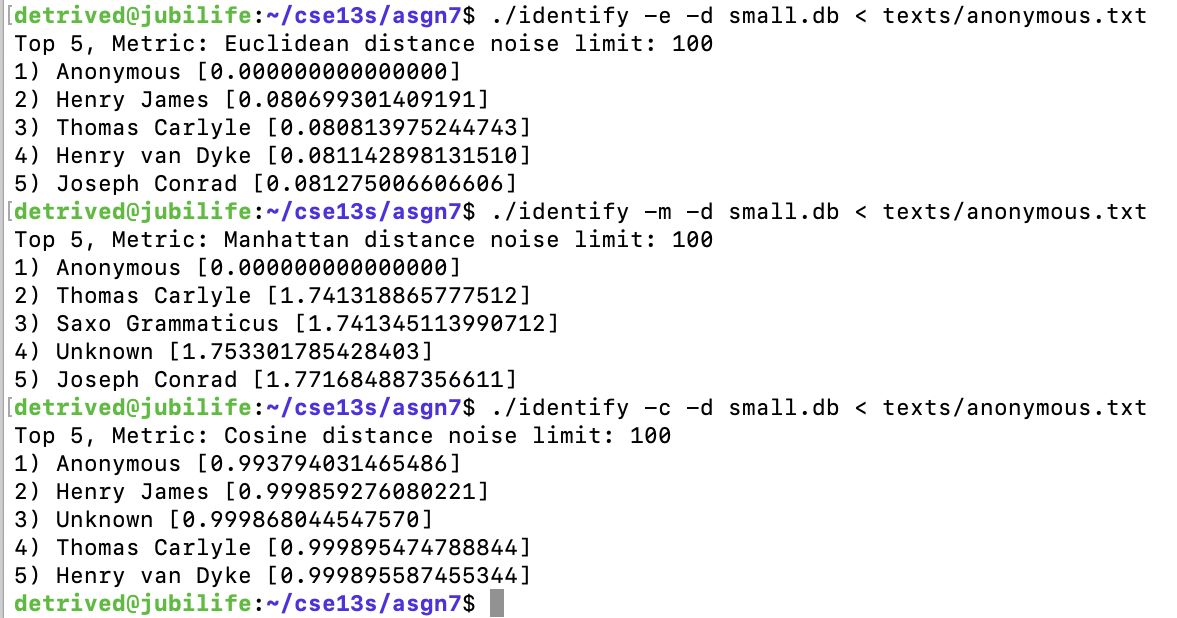
\includegraphics{ss}
\end{document}
